%----------------------------------------------------------
% PACKAGES AND THEMES
%----------------------------------------------------------
\documentclass[aspectratio=169,xcolor=dvipsnames,handout]{beamer}

\usetheme{Darmstadt}
\usecolortheme{seahorse}
\setbeamercovered{transparent}
\setbeamertemplate{footline}[frame number]

\usepackage[hangul]{kotex}
\usepackage{hyperref}
\usepackage{graphicx, array, adjustbox, makecell}

% other packages
\usepackage{natbib}
\usepackage{,float,pstricks,listings,stackengine,xcolor,calligra}
\usepackage{amsmath,amssymb,latexsym}
\usepackage{booktabs,longtable,multicol,multirow,lscape,rotating}
\usepackage{caption,subcaption}
    \newcommand{\source}[1]{\subcaption*{\raggedright 자료: {#1} } }
\usepackage{threeparttable} % Align column caption, table, and notes
\usepackage{adjustbox} % Shrink stuff
%\usepackage{showframe} % Useful for debugging

% defs
\def\cmd#1{\texttt{\color{red}\footnotesize $\backslash$#1}}
\def\env#1{\texttt{\color{blue}\footnotesize #1}}
\definecolor{deepblue}{rgb}{0,0,0.5}
\definecolor{deepred}{rgb}{0.6,0,0}
\definecolor{deepgreen}{rgb}{0,0.5,0}
\definecolor{halfgray}{gray}{0.55}

\lstset{%
    basicstyle=\ttfamily\small,
    keywordstyle=\bfseries\color{deepblue},
    emphstyle=\ttfamily\color{deepred},    % Custom highlighting style
    stringstyle=\color{deepgreen},
    numbers=left,
    numberstyle=\small\color{halfgray},
    rulesepcolor=\color{red!20!green!20!blue!20},
    frame=shadowbox,
}


% font조정
%\usepackage{fontspec}
%\setmainfont{Times New Roman}
%\setmainhangulfont{NanumGothic}

% 문자열 대체{노사관계론 전용}
\usepackage{newunicodechar}
\newunicodechar{•}{$\cdot$}
\newunicodechar{➔}{$\implies$}
\newunicodechar{∴}{$\therefore$}
\newunicodechar{∵}{$\because$}

%----------------------------------------------------------
% TITLE PAGE
%----------------------------------------------------------
\title{분배적 정의와 한국의 기회불평등}
\subtitle{}
\author{오성재}
\institute[CNU]
    {\relax
        사회보장정책연구실 세미나
    }
\date{\today}

%----------------------------------------------------------
\begin{document}
%----------------------------------------------------------

\frame{\titlepage}

\begin{frame}{목차}
    \setcounter{tocdepth}{1}
    \tableofcontents
\end{frame}

\section{분배적 정의}
\subsection{분배적 정의의 원칙들}
\begin{frame}[<+->]
\frametitle{분배적 정의의 원칙}
    \begin{itemize}
        \item 평등(equalit)의 원칙
        \item 충분성(sufficiency)의 원칙
        \item 우선(proority)의 원칙
        \item 효용(utility)의 원칙
        \item 공로(merit)의 원칙
        \item 자유(liberty)의 원칙
    \end{itemize}
\end{frame}

\begin{frame}[<+->]
\frametitle{평등의 원칙}
    \begin{itemize}
        \item 불평등은 그 자체로 정의롭지 않다. 따라서 평등 분배는 어떤 불평등 분배보다 정의롭다.
        \item 평등분배를 위해서 타인을 끌어내리는 것 역시 정당화 할 수 있다.
    \end{itemize}
    \begin{alertblock}{평등지상주의?}
    \begin{itemize}
        \item 맹인 한 사람이 존재하는 사회가 평등주의를 달성하려면?
        \item 능력이나 노력에 관계없이 모두가 동등한 결과를 얻는 사회는 정의로운가?
    \end{itemize}
    \end{alertblock}
\end{frame}

\begin{frame}[<+->]
\frametitle{충분성의 원칙, 우선의 원칙}
    \begin{itemize}
        \item 충분성의 원칙
        \begin{itemize}
            \item 모두가 \textbf{어떤 대상(basket)}을 충분하게 가지는 것이 중요하다.
            \item 소유의 상대적 비교(격차의 유무, 크기)는 중요하지 않다.
        \end{itemize}
        \item 우선의 원칙
        \begin{itemize}
            \item 분배에서 가장 열악한 위치에 처한 사람들이 개선되어야 한다.
        \end{itemize}
    \end{itemize}
\end{frame}

\begin{frame}[<+->]
\frametitle{효용의 원칙}
    \begin{itemize}
        \item 효용을 극대화 하는 분배가 정당한 분배이다.
        \item 불평등이나 빈곤의 증가는 순효용의 극대화를 위한다면 가능하다.
    \end{itemize}
    \begin{figure}
        \centering
        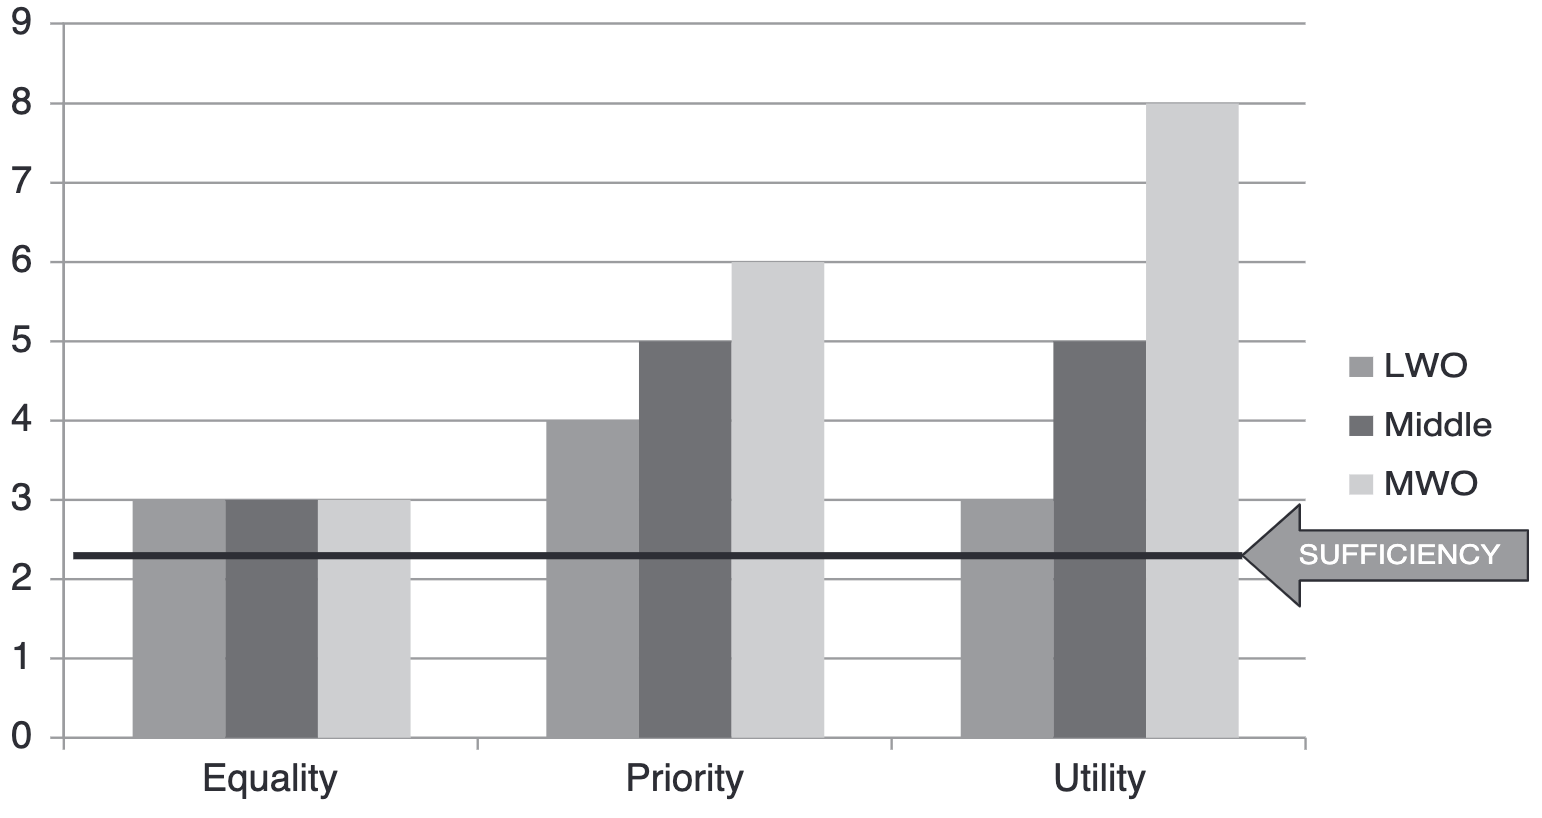
\includegraphics[width=.6\textwidth]{pic/fig1_4.png}
    \end{figure}
\end{frame}

\begin{frame}[<+->]
\frametitle{공로의 원칙, 자유의 원칙}
    \begin{itemize}
        \item 공로의 원칙
        \begin{itemize}
            \item 개인의 공로나 자격(desert)을 반영한 분배가 정당하다.
            \item 동일한 기여를 하면 같은 몫을 얻을 수 있다는 점에서 형평(equity)의 원칙으로도 볼 수 있음.
        \end{itemize}
        \item 자유의 원칙
        \begin{itemize}
            \item 정당한 분배는 사람들의 소유의 형태로 판단할 수 없다.
            \item 개인들 간에 모든 자발적 행위의 결과는 정당하다.
        \end{itemize}
    \end{itemize}
\end{frame}

\subsection{자유지상주의}%
\begin{frame}[<+->]
\frametitle{자유지상주의}
    \begin{itemize}
        \item 개인의 삶에 국가에 의한 강압적 지배가 없어야 한다는 사상 중 하나.
        \begin{itemize}
            \item 모든 개인은 자신의 행동이 평등한 타인의 자유권을 침해하지 않는 한, 스스로 무엇을 할 것인지 결정할 자유가 있음.
        \end{itemize}
        \item 국가는 구성원들의 활동의 자유가 서로 일관되게 하기 위해서만 간섭.
        \begin{itemize}
            \item 국가는 폭력, 절도, 기만 등으로부터 구성원을 보호하는 역할.
            \item 가부장적 정부 (예: 안전벨트 착용 의무화, 마약 사용 금지, 결혼에 대한 특정 견해 시행 등)의 역할을 하거나 재분배를 추구해서는 안됨.
        \end{itemize}
        \item 권위의 범위 측면에서 국가의 크기를 정의.
        \begin{itemize}
            \item 절대 군주는 백성의 생활 전체를 통제할 수 있는 강력한 권한을 가질 수 있지만 직위나 법을 만들지 않고도 가능(군주의 뜻 하나로도 가능).
        \end{itemize}
    \end{itemize}
\end{frame}

\begin{frame}[<+->]
\frametitle{소유의 정의}
    \begin{itemize}
        \item Nozick은 정부가 구성원들에게 분배해야할 대상 그 자체가 없다고 주장.
        \item 분배는 어떤 정당한 분배로부터 합법적인 수단을 통해서 이뤄질 때만 정당.
        \item 합법적인 수단은 자원의 최초 획득 그리고 재화와 용역의 이전을 규정짓는 원칙에 의해 지정.
    \end{itemize}
\end{frame}

\begin{frame}[<+->]
\frametitle{자격 이론}
    \begin{itemize}
        \item Nozick의 분배 정의는 자격의 문제; 자격을 갖추 소유만이 정의.
        \begin{itemize}
            \item 정당한 획득의 원칙 : 소유된 역사가 없는 자원의 원초적 할당에 대하여.
            \item 정당한 이전의 원칙 : 재화와 용역의 개인간 교환에 대하여.
            \item 교정의 원칙 : 위 두 원칙이 위반될 경우에 대하여.
        \end{itemize}
    \end{itemize}
\end{frame}

\subsection{고전적 자유주의}%
\begin{frame}[<+->]
\frametitle{하이에크}
    \begin{itemize}
        \item 자유시장경제에 대한 유일한 대안은 계획경제.
        \item 인간의 무지 때문에 자유 시스템은 재화와 서비스를 효율적으로 생산하고 분배하는 데 계획 경제보다 우월.
        \item 상품 및 서비스의 생산 및 유통을 위한 시스템이 더 효율적일수록 평균적인 구성원이 삶의 목적을 달성하는 데 성공할 가능성이 높아짐. 
        \item 효용과 자유의 원칙은 함께 가야.
    \end{itemize}
\end{frame}

\begin{frame}[<+->]
\frametitle{하이에크의 분배정의 원칙}
    \begin{itemize}
        \item 효용의 원칙: 정의로운 사회는 사회의 목적(효용과 자유)을 가장 잘 촉진하는 사회.
        \item 자유의 원칙: 정당한 자원의 분배는 자유 시장에서의 자발적인 거래의 결과인 분배.
        \item 충분주의 원칙: 사회가 극도의 빈곤을 허용해서는 안되며 모든 사회 구성원이 최소한의 기본 소득을 보장함으로써 만족할 수 있는 최소한의 품위 있는 삶을 영위할 수 있도록 보장해야.
    \end{itemize}
\end{frame}

\begin{frame}[<+->]
\frametitle{하이에크와 평등원칙}
    \begin{itemize}
        \item 법 앞에의 평등: 법이 특권이나 차별을 조장해선 안된다.
        \item 최소주의적 기회의 평등:
        \begin{itemize}
            \item  자연적 운(타고난 외모 및 지능)은 자유의 원칙에 위배되지 않음.
            \item  상이한 자연적 운은 경제성장의 주요한 요인.
            \item  자연적 운의 영향을 최소화 하려는 시도는 정부의 미시적 조정을 수반함.
        \end{itemize}
    \end{itemize}
\end{frame}

\subsection{자유주의적 평등주의}%
\begin{frame}[<+->]
\frametitle{공리주의(utilitarianism)에 대한 롤즈의 비판}
    \begin{itemize}
        \item \textbf{사회}를 단순히 효용 (의 구성 요소)의 생산활동을 위한 공동체로 간주.
        \item 사회 구성원인 \textbf{개인}을 일차적으로 효용의 수단으로 간주.
        \item 효용의 총합에만 초점을 맞추므로 자원, 기회, 부담 및 권리가 \textbf{어떻게} 분배되어야 하는지에 대한 설명 부족.
        \item 개인의 효용 추구에서 어떤 \textbf{기본권}이 중요한 데 공리주의는 이를 파악하지 못하고, 따라서 그 기본권을 모두에게 동등하게 보호하지 못함.
    \end{itemize}
\end{frame}
 
\begin{frame}[<+->]
\frametitle{롤즈 vs. 하이에크}
    \begin{itemize}
        \item 롤즈와 하이에크는 분배적 정의의 원칙과 이를 실현할 사회체제의 관계가 서로 상반됨.
        \begin{itemize}
            \item  롤즈는 민주사회가 정의로운 사회이고 이를 이루기 위해 분배적 정의의 원칙을 제시. 
            \item  하이에크는 정의로운 분배를 달성하기 위한 수단으로 자유시장주의와 법치주의가 필요하다는 입장. 
        \end{itemize}
    \end{itemize}
\end{frame}

\begin{frame}[<+->]
\frametitle{기본재 (primary good)}
    \begin{enumerate}
            \item  기본권과 자유.
            \item  이동의 자유와 직업 선택의 자유.
            \item  직위와 직책에 접근할 수 있는 권한, 특권 및 기회.
            \item  소득과 재산.
            \item  자존감의 사회적 기반.
    \end{enumerate}
\end{frame}

\begin{frame}[<+->]
\frametitle{정의의 원칙}
    \begin{enumerate}
        \item  동등한 기본권의 원칙: 모든 사람은 최대한의 평등한 기본 자유를 누릴 권리가 있으며, 이는 다른 사람들의 동일한 자유와 양립할 수 있어야 한다.
        \item  민주적 평등의 원칙: 
        \begin{itemize}
            \item[a] 공정한 기회 균등 원칙: 사회적, 경제적 불평등은 모든 사람에게 공정한 기회가 제공되는 조건에서만 허용된다. 즉, 같은 재능과 의지력을 가진 사람은 배경과 상관없이 동등한 기회를 가져야 한다.
            \item[b] 차등의 원칙: 불평등이 허용되는 경우, 그것은 사회의 가장 불리한 위치에 있는 사람들에게 최대의 혜택을 제공하는 방식이어야 한다.
        \end{itemize}
    \end{enumerate}
\end{frame}

\begin{frame}[<+->]
\frametitle{우선의 원칙}
    \begin{itemize}
        \item 우선 원칙: 첫 번째 원칙은 두 번째 원칙에 우선. 두 번째 원칙의 a 항목이 b 항목보다 우선.
        \item 우선순위가 낮은 원칙에 대한 큰 이익을 위해 우선순위가 높은 원칙을 타협할 수 없다는 의미.
    \end{itemize}
\end{frame}

\section{기회불평등의 이론 및 측정}%
\subsection{Equality of what?}
\begin{frame}{Dworkin(1981): 복지 평등에 대한 비판과 자원 평등}
  \begin{itemize}
    \item Equality of Welfare: 삶의 만족도(welfare)를 평등하게 분배하자는 주장
    \item Dworkin의 비판:
    \begin{itemize}
        \item 값비싼 취향(expensive tastes)에 대한 부당한 보상
        \item 만족도의 주관성 → 정책 집행 불가능
        \item 복지(welfare)를 분배 기준으로 삼는 것은 부적절
    \end{itemize}
    \item 대안으로 \textbf{자원 평등(Eqaulity of resource)}을 제시
    \begin{itemize}
        \item \textbf{Equality of Resources:} 자원(resource)의 평등한 분배
        \item 모든 개인은 동일한 \textbf{출발선(starting gate)}에서 인생을 설계해야 함
        \item \textbf{Envy Test:} 누구도 타인의 자원 묶음을 부러워하지 않는 상태가 자원평등이 달성된 상태.
    \end{itemize}
  \end{itemize}
\end{frame}

\begin{frame}{Arneson의 평등 이론}
  \begin{itemize}
        \item Dworkin의 자원 평등론에 대한 비판.
  \begin{itemize}
        \item ‘재능의 노예(slavery of the talented)’문제: 재능이 많은 사람이 오히려 개인 자유를 잃고 불리해질 수 있음.
        \item 자원 평등은 이러한 개인적 특성을 제대로 보상하지 못함.
  \end{itemize}
    \item \textbf{Equal Opportunity for Welfare:} 후생을 실현할 수 있는 기회의 평등
  \begin{itemize}
        \item 후생 수준의 불평등은 허용되지만, \textbf{기회 자체의 불평등은 허용 불가}
        \item 개인의 선호는 이성적 숙고 후의 선호(ideally considered preferences)로 측정되어야.
        \item 개인이 통제 불가능한 조건에 기초한 복지 차이는 보상되어야. 
  \end{itemize}
  \end{itemize}
\end{frame}

\begin{frame}{Cohen의 평등 이론}
  \begin{itemize}
    \item Dworkin 비판: 자원만으로는 \textbf{실질적 불이익}(고통, 무능력)을 설명 불가
    \begin{itemize}
        \item 평등주의는 \textbf{운(bad luck)}으로 인한 불리함을 제거하려는 윤리적 충동에서 비롯됨.
        \item Dworkin은 “자원”이라고 했지만, 실제로는 ‘선택 vs. 운’의 구분이 핵심.
    \end{itemize}
    \item \textbf{Equal Access to Advantage}: 삶에서의 이익 전체(advantage)를 고려
    \begin{itemize}
            \item 순응적 주부(tamed housewife) 문제.
            \item 고통, 장애, 선천적 한계 등도 \textbf{공정한 분배 고려 요소}로 포함해야.
    \end{itemize}
  \end{itemize}
\end{frame}

\begin{frame}{Roemer의 기회평등 이론}
  \begin{itemize}
    \item 개인의 성과(outcome)는 \textbf{환경(circumstance) + 노력(effort) + 정책(policy)}의 함수
    \begin{itemize}
        \item 성과는 교육, 경제력, 건강과 같은 분야에서 개인이 획득한 성취.
        \item 환경은 개인이 선택할 수 없으면서 성취에 영향을 미치는 요소(가정환경, SES, 유전적 요인).
        \item 순수한 노력의 문제 : 환경의 영향을 받지 않는 노력으로 측정해야
        \item 정책은 \textbf{결과가 노력에만 따라 결정되도록} 설계 되어야.
    \end{itemize}
  \end{itemize}
\end{frame}

\subsection{기회불평등 측정}
\begin{frame}{기회평등의 정의}
  \begin{itemize}
    \item 엄밀한 기회평등은 성취 $y$의 확률분포 $y=F(y|c)$가 임의의 두 환경 $c,c' \in C$에 대해 $F(\cdot | c) = F(\cdot | c')$가 성립함을 요구.
    \item 기회균등기저에 속한 어떤 두 환경 간에 제1차 혹은 제2차 확률지배관계가 존재할 경우 기회불평등이 존재하며 이러한 관계가 없을때 (완화된)기회평등 사회로 정의.
    \begin{itemize}
        \item 제1차 기회불평등 조건: 어떤 두 환경 $c,c' \in C$에 대하여 $F(y | c)$와 $F(y | c')$사이에 제1차 확률지배관계가 성립한다.
        \item 제2차 기회불평등 조건: 어떤 두 환경 $c,c' \in C$에 대하여 $F(y | c)$와 $F(y | c')$사이에 제2차 확률지배관계가 성립한다.
    \end{itemize}
  \end{itemize}
\end{frame}

\begin{frame}{지니 기회불평등 지수}
  \begin{itemize}
    \item 기회불평등한 사회 간에도 정도의 비교가 필요.
    \item \citet{letl08}은 불평등 지수로 널리 쓰이는 지니계수에서 착안한 지수를 활용. 총 $k$개의 환경이 있고 환경 가치의 평균값을 $\mu$라고 하면, 각 환경 $t$의 비중이 $P_t$일 때, 지니 기회불평등지수는 다음 식과 같이 정의됨.
    \begin{equation}
        G O=\frac{1}{\mu} \sum_{i=1}^{k} \sum_{j>i} P_{i} P_{j}\left(\mu_{j}\left(1-G_{j}\right)-\mu_{i}\left(1-G_{i}\right)\right).
        \label{eq:goms_GOI}
    \end{equation}
  \end{itemize}
\end{frame}

\begin{frame}{개천용 지수}
  \begin{itemize}
        \item 열악한 환경에서도 최상위 성취전망이 높은 사회에서는 계층상승의 기회가 크다고 할 수 있고, 최하위에서 최상위로의 계층상승의 전망을 반영하는 지표도 기회불평등지표로 유용하게 활용 가능.
        \item 가장 열악한 환경 $\underline{c}$에 처한 사람들의 전체인구에서의 비율을 $q_{\underline{c}}$이라 하고, 최상위 성취 집단을 소득 상위 $p$퍼센트에 속하는 사람들이라고 하고 이들의 수를 $n_p$라고 하자.
        \begin{equation}
            R R_{p}=1-\frac{n_{p, \underline{c}} / n_{p}}{q_{\underline{\underline{c}}}}.
            \label{eq:goms_RRI}
        \end{equation}
        \item 예를 들어 개천용불평등지수가 0.6인 사회에서는 최악의 환경에서 성공할 수 있는 100명중에서 60명이 기회불평등 때문에 실패.
    \end{itemize}
\end{frame}

\section{한국의 교육기회불평등}%
\begin{frame}{연구 배경}
  \begin{itemize}
    \item 계층이동성 인식 악화, 교육 격차 심화 
    \item 교육이 계층사다리 기능을 하지 못한다는 인식
    \item 대학입시 유형(정시/수시)에 따라 교육기회불평등 차이 존재
    \item 정시 확대 정책의 효과 검토 필요
  \end{itemize}
\end{frame}

\begin{frame}{자료 소개: GOMS}
  \begin{itemize}
    \item 한국고용정보원 대졸자직업이동경로조사 (2007--2017)
    \item 약 18,000명/년 반복횡단면 자료
    \item 주요 변수 : 졸업대학, 부모 학력$\cdot$소득, 성별, 고교지역, 대입전형유형
  \end{itemize}
\end{frame}

\begin{frame}{기초 통계 및 변수 정의}
  \begin{itemize}
    \item 대학성취 점수: QS 순위 및 학제 기반 50개 대학을 1--5점척도로 환산(5점: 1--10위 대학)
    \item 가구환경지수: 부모 학력 및 소득을 기반으로 주성분분석(PCA)로 종합화 후 세 유형으로 구분
    \item 고교지역: 수도권, 광역시, 기타 도지역
    \item 대입유형: 정시, 수시 (특별전형 제외)
  \end{itemize}
\end{frame}

\begin{frame}{기초 통계: 주성분분석환경 구성비율}
    \centering
    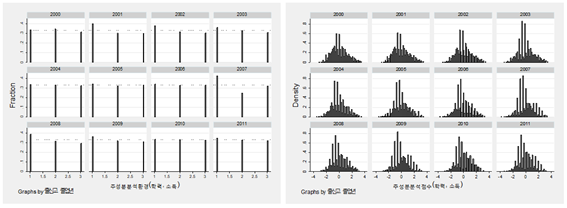
\includegraphics[width=0.8\textwidth]{figure/goms_pca.png}
\end{frame}

\begin{frame}{대학입학 성취의 누적분포}
  \centering
  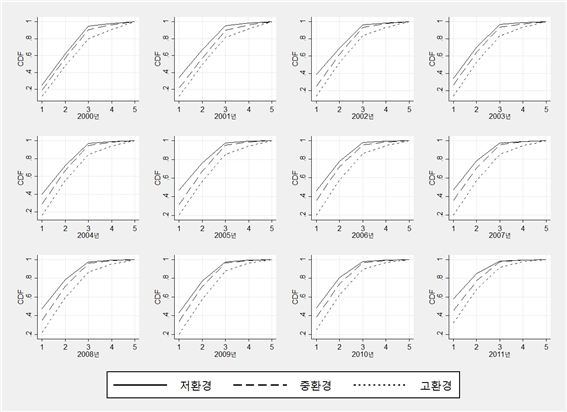
\includegraphics[width=0.6\textwidth]{figure/goms_cdf_bypca.png}
\end{frame}

\begin{frame}{지역환경별 누적분포}
  \centering
  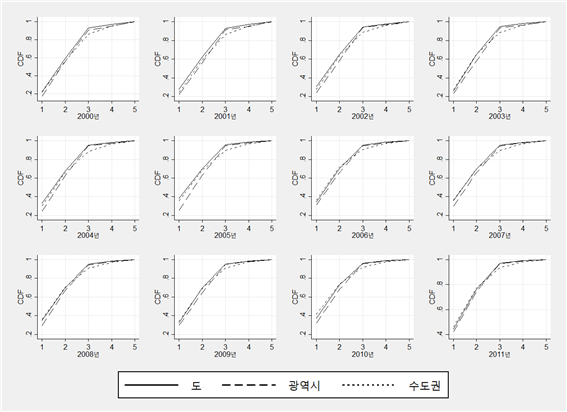
\includegraphics[width=0.6\textwidth]{figure/goms_cdf_byrgn.png}
\end{frame}

\begin{frame}{전공유형별 누적분포 비교}
  \centering
  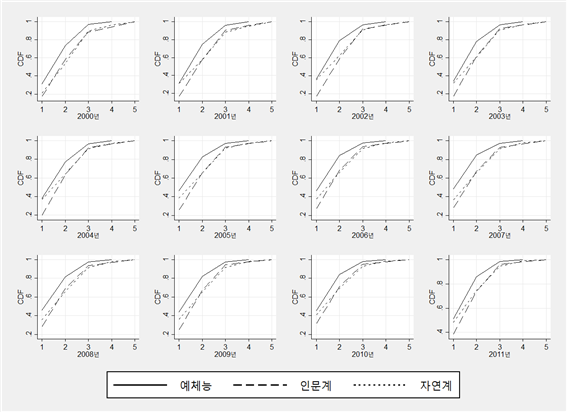
\includegraphics[width=0.6\textwidth]{figure/goms_cdf_bysex.png}
\end{frame}

\begin{frame}{GOI 지수 추이: 환경별}
  \centering
  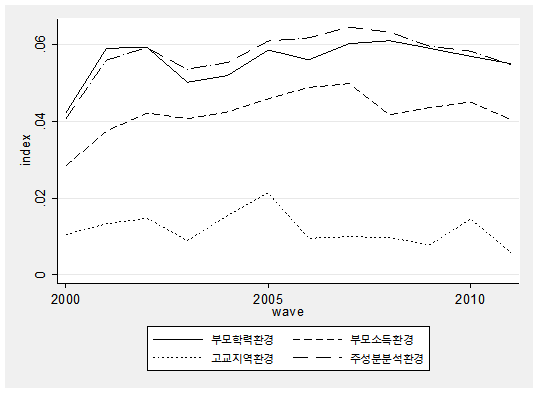
\includegraphics[width=0.6\textwidth]{figure/goms_goi_byenv.png}
\end{frame}

\begin{frame}{GOI 지수 추이: 입시유형별}
  \centering
  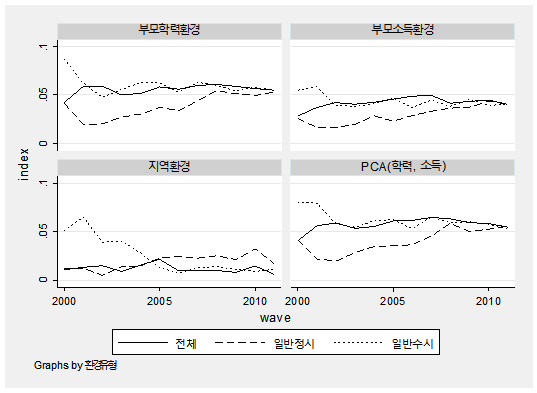
\includegraphics[width=0.6\textwidth]{figure/goms_goi_byent.png}
\end{frame}

\begin{frame}{RRI 지수 추이: 입시유형별}
  \centering
  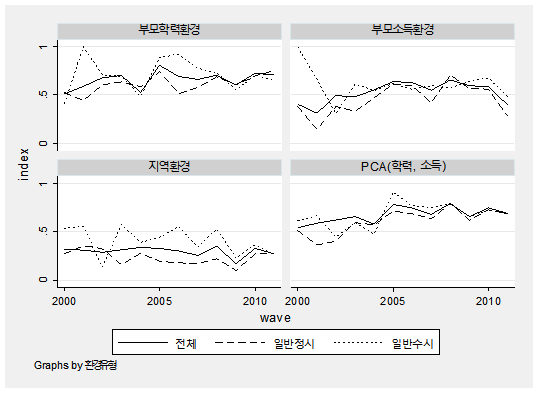
\includegraphics[width=0.6\textwidth]{figure/goms_rri_byent.png}
\end{frame}

\begin{frame}{결론 및 시사점}
  \begin{itemize}
    \item 대학입학에 뚜렷한 기회불평등 존재
    \item 부모의 학력/소득이 주요한 기저요인
    \item 정시보다 수시 전형에서 기회불평등 높음 $\rightarrow$ 제도 설계 필요
    \item 지역균형전형 강화 필요
    \item GOI, RRI 지수는 정책 모니터링에 유용
  \end{itemize}
\end{frame}

\begin{frame}{참고 : 부친학력별 수능점수 분포}
  \centering
  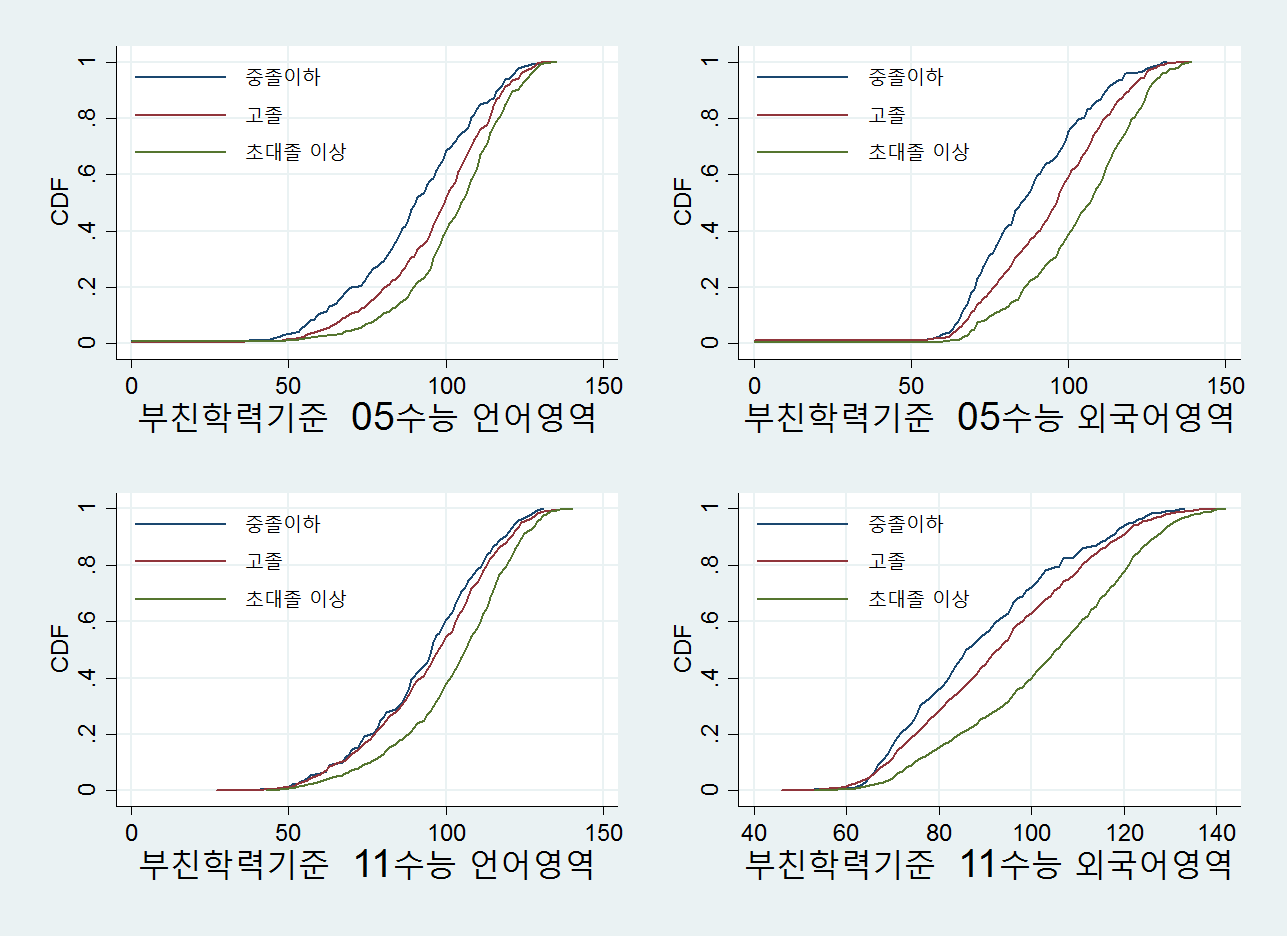
\includegraphics[width=0.6\textwidth]{figure/KELS_y56edugrp.png}
\end{frame}

\begin{frame}{참고 : 부친학력별 자습시간 분포}
  \centering
  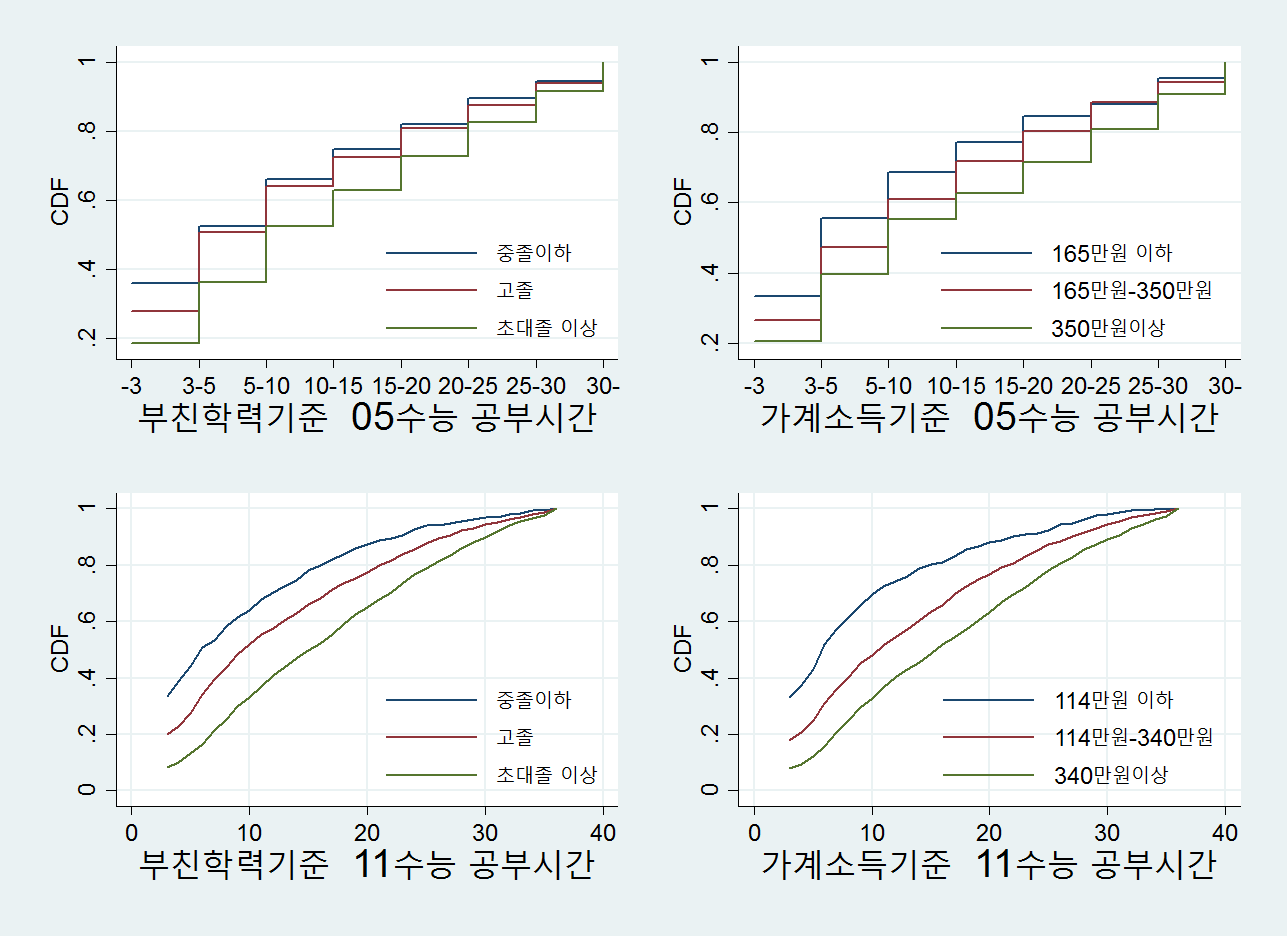
\includegraphics[width=0.6\textwidth]{figure/KELS_y56hurgrp.png}
\end{frame}

\begin{frame}{참고 : 부친학력별 사교육비 분포}
  \centering
  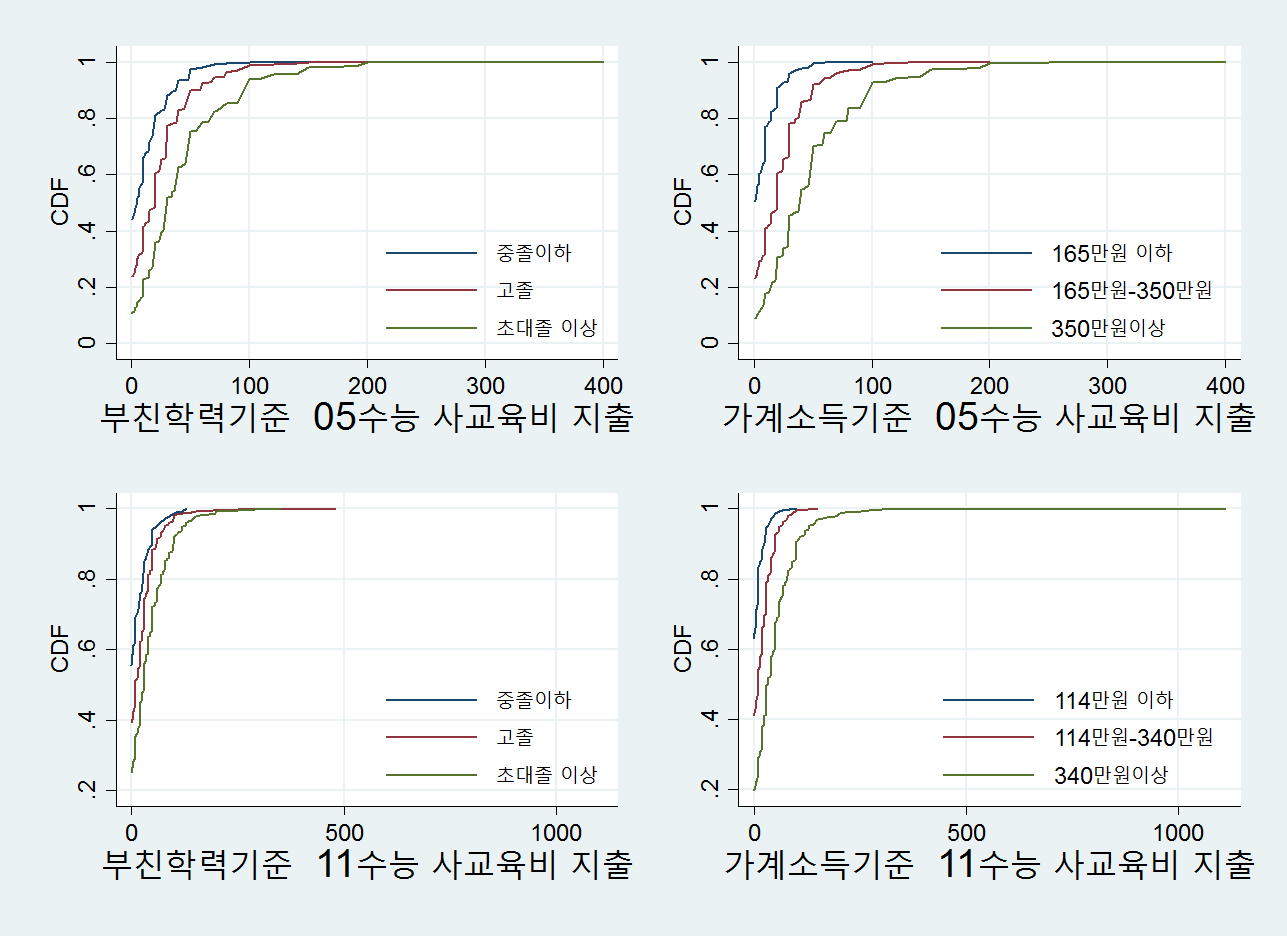
\includegraphics[width=0.6\textwidth]{figure/KELS_y56pedgrp.png}
\end{frame}

\begin{frame}{참고 : 출신지역별 수능점수 분포}
  \centering
  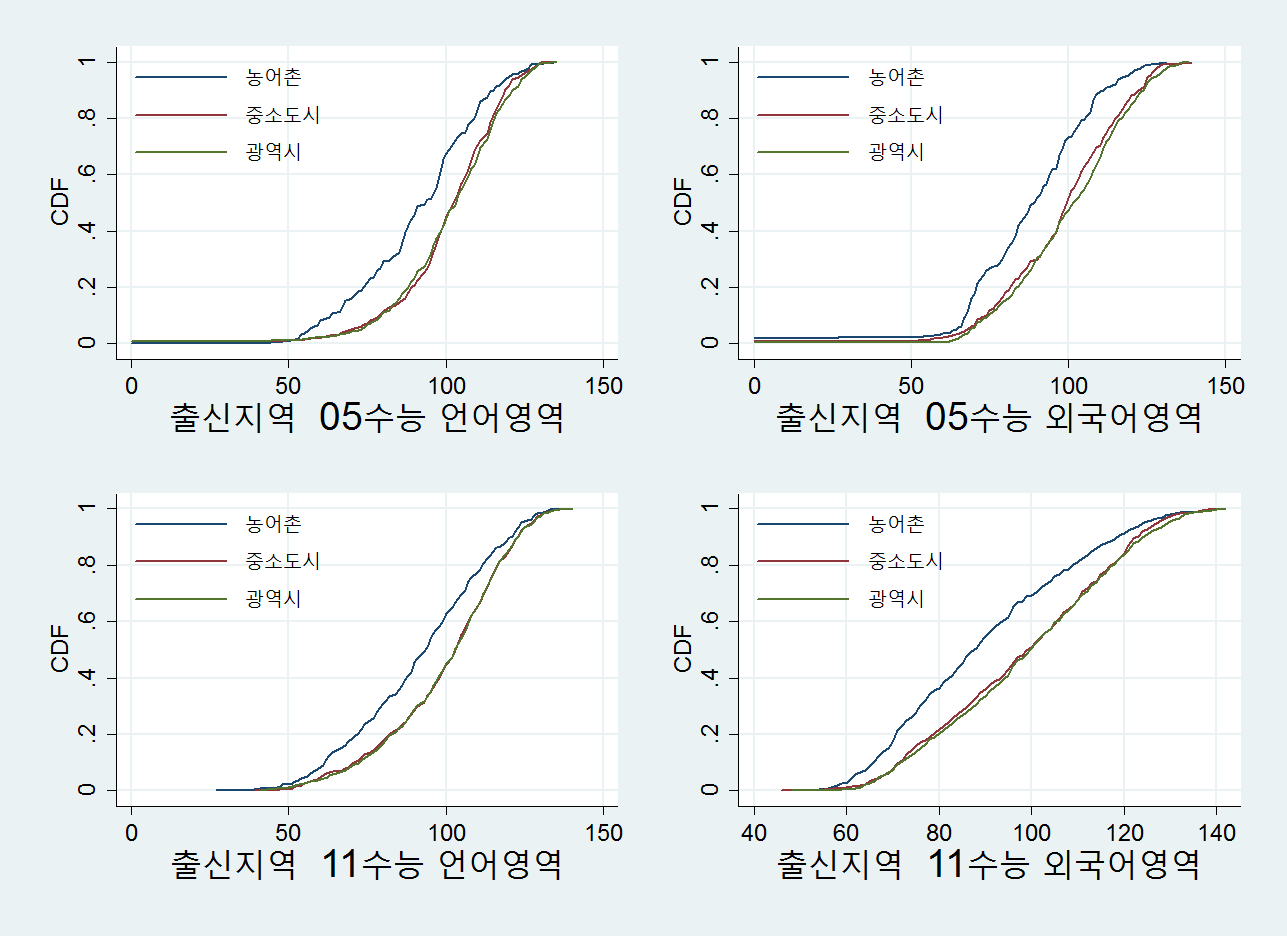
\includegraphics[width=0.6\textwidth]{figure/KELS_y56reggrp.png}
\end{frame}

\section{한국의 소득기회불평등}%

\begin{frame}{자료 소개: KLIPS}
  \begin{itemize}
        \item 한국노동연구원 한국노동패널 (1998--2019)
        \item 2019년 자료 기준 전국 12,000여 가구 23,000 여명.
        \item 주요 변수 : 가계 총소득, 가구주 부친의 학력, 가구주 부친의 직업력 등등.
        \item 가계 총소득은 년도효과 통제를 위해 2개년 평균치를 사용.
        \item 가구주의 연령 기준으로 전연령 및 30--50세로 구분하여 분석.
  \end{itemize}
\end{frame}

\begin{frame}{가구소득의 누적분포: 가구주부친직업환경, 가구주연령 30---50세}
  \centering
    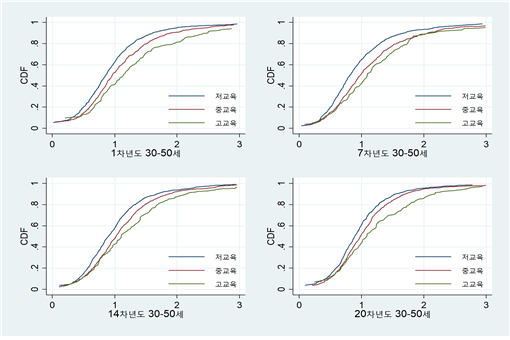
\includegraphics[scale=.5]{figure/klips_cdf4_byjob.png}
\end{frame}

\begin{frame}{가구소득의 확률분포: 가구주부친직업환경, 가구주연령 30---50세}
    \centering
    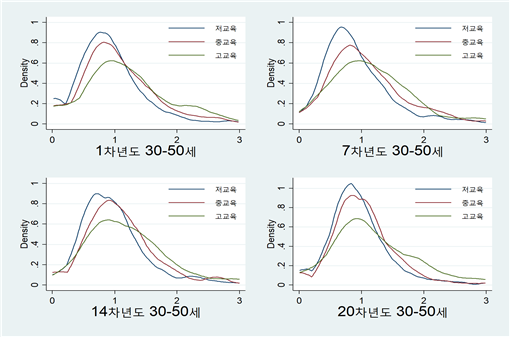
\includegraphics[scale=.5]{figure/klips_pdf4_byjob.png}
\end{frame}

\begin{frame}{기회불평등지수 추이: 가구주부친학력환경}
    \centering
    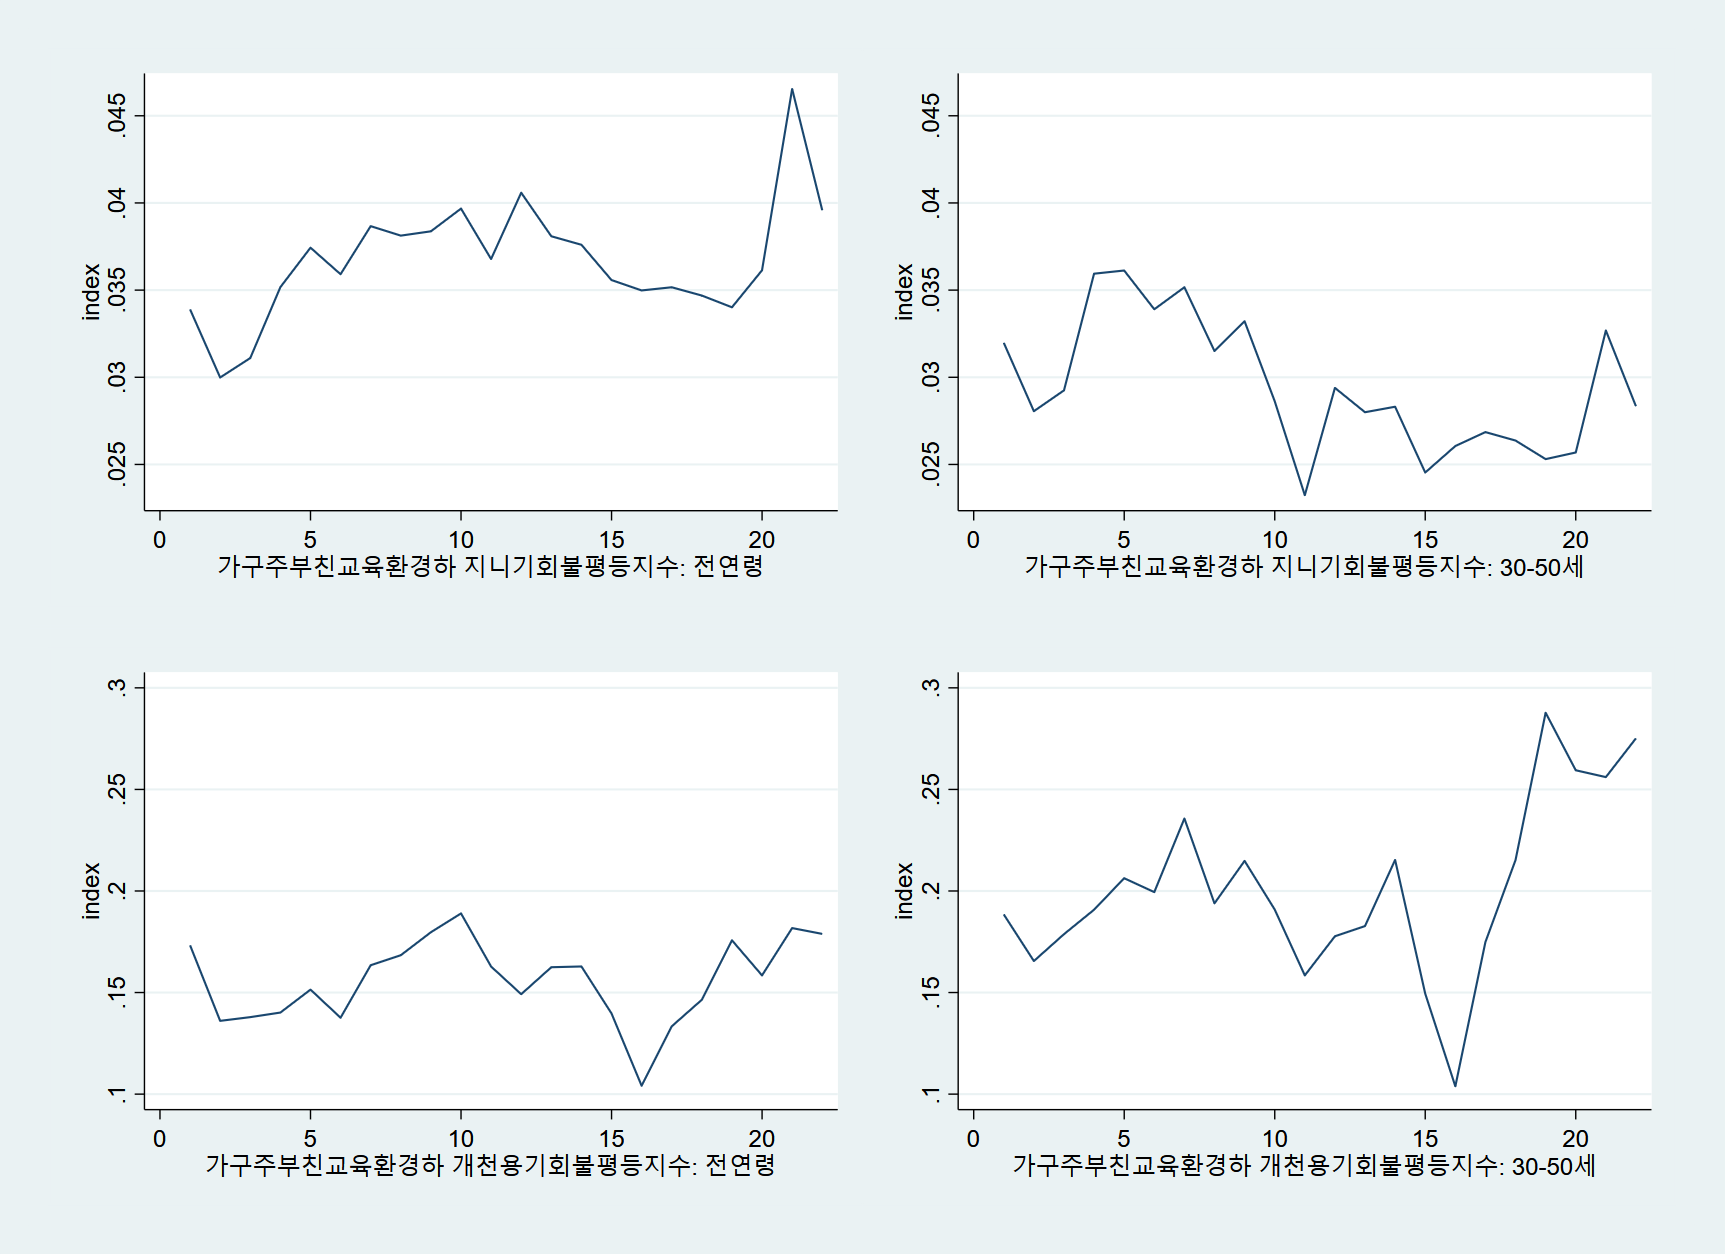
\includegraphics[width=.6\textwidth]{figure/incn1m_edugrp_index.png}
\end{frame}

\begin{frame}{결론 및 시사점}
  \begin{itemize}
    \item 가구총소득에 뚜렷한 기회불평등 존재
    \item 가구주 부모의 학력이 주요한 기저요인
    \item 산업화와 교육의 양적 확대에 힘입어 중장년층이 더 기회를 많이 누린 것으로 나타남.
    \item 최근년의 높은 개천용 지수의 상승은 우리 사회가 체감하는 높은 기회불평등이 주요 경제활동연령층이 경제적 성공을 얻는데 대한 기회불평등임을 시사.
  \end{itemize}
\end{frame}

\section{교육기회불평등과 경제성장}%

\subsection{문제제기}
\begin{frame}
    \begin{itemize}
        \item 불평등과 경제성장의 단기 관계에 대한 실증연구는 다양한 결과를 제시함.
    \end{itemize}
    \begin{figure}[htpb]
        \begin{center}
            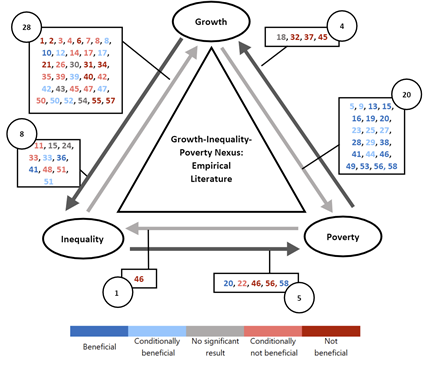
\includegraphics[scale=0.35]{fig/triangle_relations.png}
            \source{\cite{cetl21}} 
        \end{center}
    \end{figure}
\end{frame}

\subsection{선행연구}

\subsubsection{불평등과 경제성장}
\begin{frame}{경제적 불평등이 경제성장에 미치는 효과}
    \begin{itemize}
        \item 이론적 연구
        \begin{itemize}
            \item 물적 자본.
            \item 인적 자본(\cite{gnz93}).
            \item 소득재분배(\cite{anr94}; \cite{pnt94}).
            \item 정치 불안정 등등.
        \end{itemize}
        \item 실증적 연구
        \begin{itemize}
            \item 횡단면 자료.
            \item 국가별 패널자료.
            \item 국가별 패널자료 $+$ 기타 고려사항.
        \end{itemize}
    \end{itemize}
\end{frame}

\begin{frame}{실증연구의 동향}
    \begin{itemize}
        \item 횡단면 자료: \cite{barro91}, \cite{anr94}, \cite{pnt94}
        \begin{itemize}
            \item 불평등은 경제성장에 부의 영향
        \end{itemize}
        \item 국가별 패널자료: \cite{lnz98}, \cite{barro20}, \cite{forbes00}, \cite{bnd03}
        \begin{itemize}
            \item 효과의 방향이 불확실, 부/영/정의 영향
        \end{itemize}
        \item 국가별 패널자료 + 국가별 이질성 및 세부 구성요인:
        \begin{itemize}
            \item \cite{voit05, voit11}: 중상위 불평등, 중하위 불평등
            \item \cite{cc10}: 중/저소득 vs. 고소득 국가 집단
            \item \cite{hetl14}: 단기 vs. 장기
        \end{itemize}
    \end{itemize}
\end{frame}

\subsection{연구방법}
\subsubsection{기회불평등지수}
\begin{frame}{기호}
    \begin{itemize}
        \item  $i$ : 개인, $(i \in \{1,\ldots,N \} )$.
        \item 환경변수 $C_{ic}$ : 개인 $i$의 성취에 영향을 주면서 그 개인이 스스로의 의지로 선택할 수 없는 요인.(부모의 소득, 학력, 인종, 성별 등등.).
        \item 환경 $C_i$ : 개인 $i$가 속한 환경변수$C_{ci}$ 들의 c-터플(c-turple) $C_i = (C_{1i}, \ldots , C_{ci})$. 
        \item 환경유형 $T= \{1, \ldots , t \}$, $t= ||C_1|| \times \cdots \times ||C_c||$ : 가능한 모든 환경의 지표(index).
    \end{itemize}
\end{frame}

\begin{frame}{성취, 환경 그리고 노력}
    \begin{itemize}
        \item 개인 $i$의 성취인 성적점수를 $y_i$, 그가 속한 환경을 $C_i$, 노력을 $e_i$라고 표시하자.
        \item 기회불평등의 관점에서 성취는 개인이 속한 환경 및 환경과 무관한 개인의 노력의 결과라고 정의한다.
        \item 개인 $i$ 성취 $y_i$는 환경 $C_i$ 및 노력 $e_i$에 대하여 다음의 선형함수관계를 가진다고 가정한다.
        \begin{equation}
            \label{eq:ols}
             y_{i} =\beta _0 +  \beta _1 C_{1i} + \cdots + \beta _c C_{ci} + \epsilon _i
        \end{equation}
    \end{itemize}
\end{frame}

\begin{frame}{\cite{fng11}}
    \begin{itemize}
        \item 성취의 불평등을 기회의 불평등과 노력의 불평등으로 분해하기 위해 가산적 분해가능성(additively decomposibility)이 있는 타일-0(Theil-0) 지수를 이용한다.
        \begin{equation}
            \label{eq:theil0}
            T(Y)=\frac{1}{N} \sum_{i=1}^{N} \ln \left(\frac{\bar{y}}{y_{i}}\right)
        \end{equation} 
        \item \cite{fng11}는 식 (\ref{eq:ols})을 식 (\ref{eq:theil0})에 대입하는 방법으로 기회불평등과 잔여불평등을 구분한다.
    \end{itemize}
    \begin{equation}
        \label{eq:theil0-decompose}
        T(Y)=T(C ' \cdot \beta) + T(\epsilon)
    \end{equation}
\end{frame}

\begin{frame}{순수한 노력}
    \begin{itemize}
        \item \cite{betl12}는 \cite{Roemer98}의 순수한 노력(pure effort) 개념을 도입하여 식 (\ref{eq:ols})에서 오차항에 존재하는 환경의 영향을 받는 성취를 탐색.
        \item 오차항이 환경의 영향을 받는다면 조건부 분산 $\sigma ^2 _c = Var[\epsilon |C_c]$이 환경별로 상이.
        \item 잔차의 총분산이 $\sigma ^2 =  \sum _c f_c \sigma ^2 _c$인 점을 이용해 오차항의 이분산성을 해소.
        \begin{equation}
            \label{eq:theil0-bjork}
            T(Y)=T(C' \cdot \beta +\widetilde{\epsilon}) + T ( u )
        \end{equation}
        \item 위 식의 우변 첫번째 항은 기회의 불평등을 나타내고 두번째 항은 노력의 불평등이다.
    \end{itemize}
\end{frame}

\subsubsection{회귀분석모형}
\begin{frame}{회귀분석모형}
   \begin{itemize}
       \item  본 연구에서 우리는 성장 회귀분석(growth regression)에서 일반적으로 사용하는 다음의 실증모형을 추정한다.
       \item 회귀분석은 선형회귀분석(OLS), 패널 고정효과(fixed effect) 모형, 시스템 GMM(\cite{bnb98}) 방법을 적용함으로써 주요 계수들을 추정한다.
       \begin{equation}
            \begin{aligned}
            \ln \left(Y_{i, t^{\prime}}\right)-\ln \left(Y_{i, t}\right)=& \delta_{1} I O P_{i, t}+\delta_{2} I O E_{i, t}+\beta_{1} \ln \left(Y_{i, t}\right) \\
            &+X_{i, t} \beta_{2} +\alpha_{i}+\tau_{t^{\prime}}+u_{i, t^{\prime}}
            \end{aligned}
            \label{eq:regbase}
       \end{equation} 
   \end{itemize} 
\end{frame}
 
\begin{frame}{회귀분석모형의 기호}
   \begin{itemize}
        \item $i$ : 국가, $t$ : 교육기회불평등의 측정연도
        \item $t'$ : TIMSS의 경우 $t'=t+4$, PISA의 경우  $t'=t+3$
        \item $Y_{i,t}$ : 국가 $i$의 연도 $t$현재 1인당 GDP
        \item $IOP_{i,t}$ : 기회불평등 지수, $IOE_{i,t}$ : 노력 불평등의 지수
        \item $X_{i,t}$ : 국가 $i$의 $t$연도 현재 특성변수들(인구 수 및 투자재의 가격)의 벡터 
        \item $\alpha _i$ : 국가 고정효과, $\tau _{t'}$ : 연도 고정효과
   \end{itemize} 
\end{frame}

\subsection{자료소개}
\begin{frame}{TIMSS \& PISA}
    \begin{itemize}
        \item TIMSS (Trends in International Mathematics and Science Study)
        \begin{itemize}
            \item 1995, 1999, 2003, 2007, 2011, 2015, 2019년도 조사
            \item 수학/과학 학업(curriculum)성취도 검사
            \item 4학년과 8학년 학생들을 대상으로 시행.
        \end{itemize}
         \item PISA (Programme for International Student Assessment)
        \begin{itemize}
            \item 2000, 2003, 2006, 2009 , 2012, 2015, 2018년도 조사
            \item 읽기/수학/과학 문해력(literacy) 검사
            \item 만 15세 대상으로 시행.
        \end{itemize}
    \end{itemize}
\end{frame}

\begin{frame}{추가 자료설명}
    \begin{itemize}
        \item Penn World Table로부터 국가별 1인당 GDP 및 인구, 투자재의 가격 등 거시 통제변수 구축.
        \item 공통사항
        \begin{itemize}
            \item 학생의 개인/가정/교사/학교 정보 조사.
            \item 각 조사마다 34-77개 국가 참가, 총 98개국의 성적 자료.
            \item 전세계 참여학생의 수학성적을 평균 500 분산 100점으로 정규화.
        \end{itemize}
    \end{itemize}
\end{frame}

\begin{frame}{환경변수}
    \begin{itemize}
    \item 부친 및 모친의 학력 :
    \begin{itemize}
        \item ISCED Lv에 따라 분류(1-7)를 단순 합산하여 2-14의 값을 취함.
    \end{itemize}
    \item 장서수 :
    \begin{itemize}
        \item (1) 10권 미만 -- (5) 200권 초과
    \end{itemize}
    \item 가정내 소유물
    \begin{itemize}
        \item 책상, 학생방, 컴퓨터, 인터넷 등 4개 항목을 더미로 조사하여 합산(0-4)
    \end{itemize}
    \item 최대 325개(=13$\times$5$\times$5)의 독립적인 환경 조합을 구성하여 기회불평등의 비중 계산
    \end{itemize}
\end{frame}

\begin{frame}{PISA와 TIMSS의 자료 차이: 응답률}
\begin{columns}
    \begin{column}{.5\textwidth}
        \begin{figure}
            \centering
            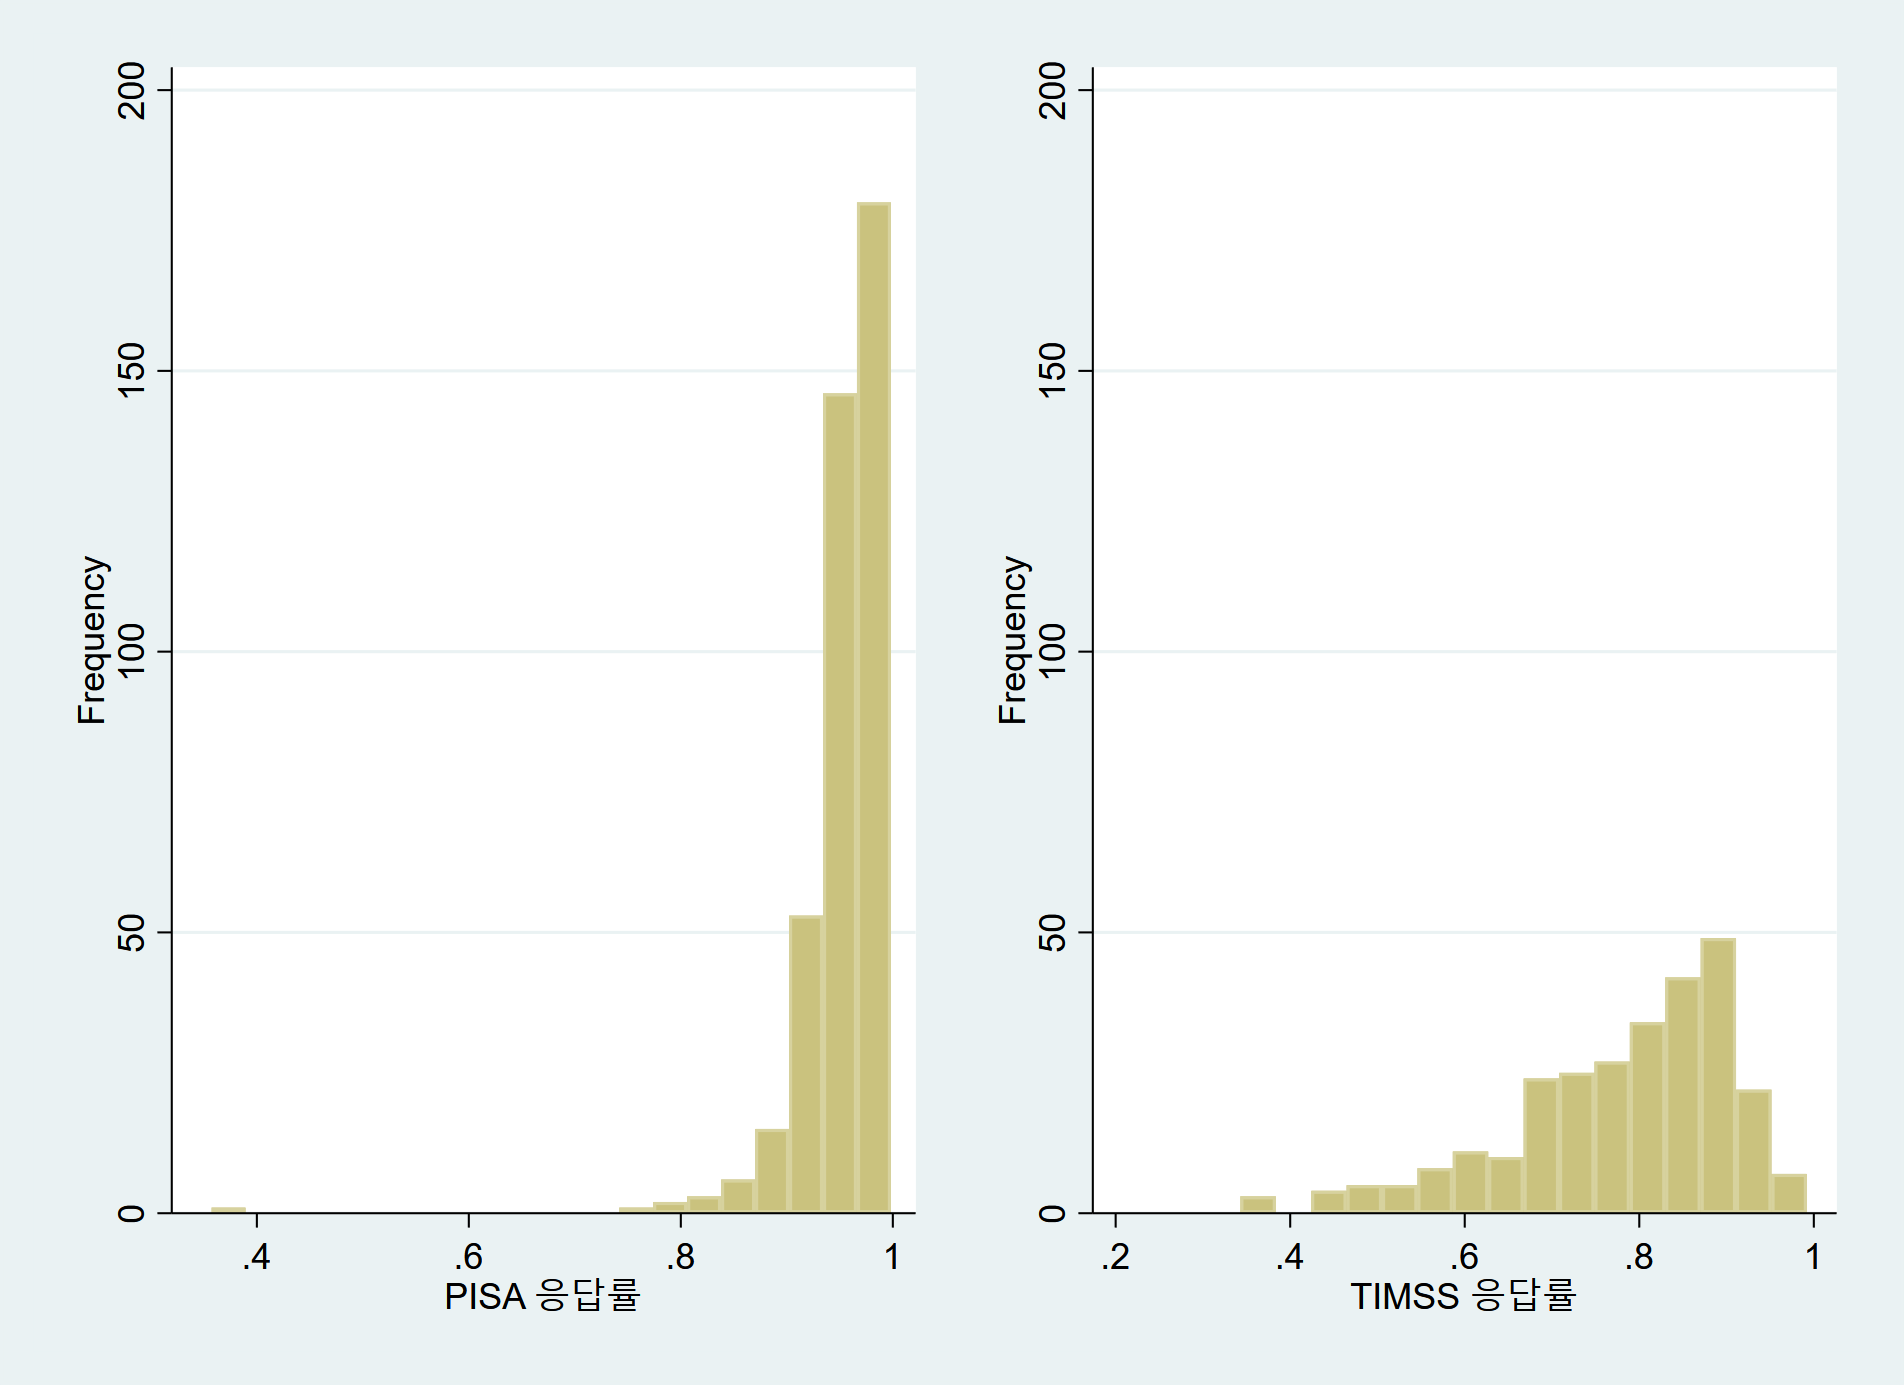
\includegraphics[scale=0.08]{fig/pnt_response.png}
            \caption{PISA와 TIMSS 환경변수 응답률}
        \end{figure}
    \end{column}    
    \begin{column}{.5\textwidth}
        \begin{itemize}
            \item TIMSS의 경우 학생이 자신의 가정환경을 응답하므로 환경변수를 활용하는 본 연구는 해당자료 사용에서 응답률의 문제를 안고 있음.
        \end{itemize}
    \end{column}    
\end{columns}
\end{frame}


\begin{frame}{PISA와 TIMSS의 자료 차이: 학업성취도 vs. 문해력}
\begin{columns}
    \begin{column}{.5\textwidth}
        \begin{figure}
            \centering
            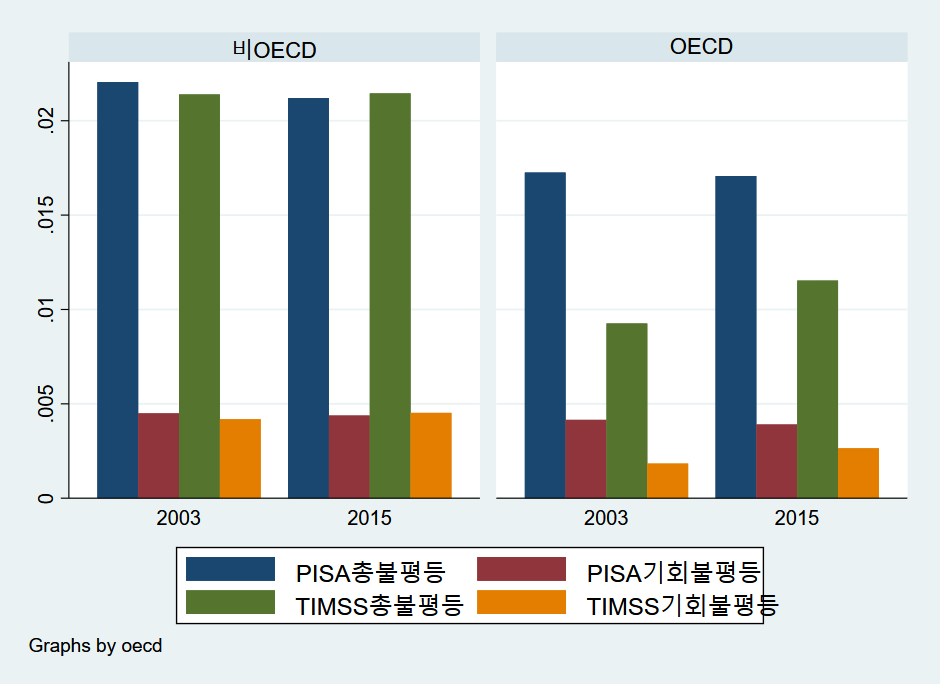
\includegraphics[scale=0.2]{fig/bar_pntcompare.png}
            \caption{PISA와 TIMSS 불평등 비교}
        \end{figure}
    \end{column}    
    \begin{column}{.5\textwidth}
        \begin{itemize}
            \item 국가별 성적의 평균을 중심으로 살펴볼때 학업성취도와 문해력은 매우 밀접한 관계를 보임.
            \item 국가별 성적의 분포를 중심으로 살펴보면 교육제도가 잘 갖춰진 국가일수록 두 교육성취는 차이를 보임. 
        \end{itemize}
    \end{column}    
\end{columns}
\end{frame}

\subsection{교육불평등지수}
\begin{frame}
    \begin{figure}[htpb]
        \begin{center}
            \includegraphics<1| handout:1>[scale=0.15]{fig/map_bjtpisa_mean.png}
            \includegraphics<2| handout:0>[scale=0.15]{fig/map_bjtpisa_2000.png}
            \includegraphics<3| handout:0>[scale=0.15]{fig/map_bjtpisa_2003.png}
            \includegraphics<4| handout:0>[scale=0.15]{fig/map_bjtpisa_2006.png}
            \includegraphics<5| handout:0>[scale=0.15]{fig/map_bjtpisa_2009.png}
            \includegraphics<6| handout:0>[scale=0.15]{fig/map_bjtpisa_2012.png}
            \includegraphics<7| handout:0>[scale=0.15]{fig/map_bjtpisa_2015.png}
            \includegraphics<8| handout:0>[scale=0.15]{fig/map_bjtpisa_2018.png}
            \caption{PISA 총불평등}
        \end{center}
    \end{figure}
\end{frame}

\begin{frame}
    \begin{figure}[htpb]
        \begin{center}
            \includegraphics<1| handout:1>[scale=0.15]{fig/map_bjrpisa_mean.png}
            \includegraphics<2| handout:0>[scale=0.15]{fig/map_bjrpisa_2000.png}
            \includegraphics<3| handout:0>[scale=0.15]{fig/map_bjrpisa_2003.png}
            \includegraphics<4| handout:0>[scale=0.15]{fig/map_bjrpisa_2006.png}
            \includegraphics<5| handout:0>[scale=0.15]{fig/map_bjrpisa_2009.png}
            \includegraphics<6| handout:0>[scale=0.15]{fig/map_bjrpisa_2012.png}
            \includegraphics<7| handout:0>[scale=0.15]{fig/map_bjrpisa_2015.png}
            \includegraphics<8| handout:0>[scale=0.15]{fig/map_bjrpisa_2018.png}
            \caption{PISA 기회불평등의 비중}
        \end{center}
    \end{figure}
\end{frame}

\begin{frame}
    \begin{figure}[htpb]
        \begin{center}
            \includegraphics<1| handout:1>[scale=0.15]{fig/map_bjttimss_mean.png}
            \includegraphics<2| handout:0>[scale=0.15]{fig/map_bjttimss_1995.png}
            \includegraphics<3| handout:0>[scale=0.15]{fig/map_bjttimss_1999.png}
            \includegraphics<4| handout:0>[scale=0.15]{fig/map_bjttimss_2003.png}
            \includegraphics<5| handout:0>[scale=0.15]{fig/map_bjttimss_2007.png}
            \includegraphics<6| handout:0>[scale=0.15]{fig/map_bjttimss_2011.png}
            \includegraphics<7| handout:0>[scale=0.15]{fig/map_bjttimss_2015.png}
            \includegraphics<8| handout:0>[scale=0.15]{fig/map_bjttimss_2019.png}
            \caption{TIMSS 총불평등}
        \end{center}
    \end{figure}
\end{frame}

\begin{frame}
    \begin{figure}[htpb]
        \begin{center}
            \includegraphics<1| handout:1>[scale=0.15]{fig/map_bjrtimss_mean.png}
            \includegraphics<2| handout:0>[scale=0.15]{fig/map_bjrtimss_1995.png}
            \includegraphics<3| handout:0>[scale=0.15]{fig/map_bjrtimss_1999.png}
            \includegraphics<4| handout:0>[scale=0.15]{fig/map_bjrtimss_2003.png}
            \includegraphics<5| handout:0>[scale=0.15]{fig/map_bjrtimss_2007.png}
            \includegraphics<6| handout:0>[scale=0.15]{fig/map_bjrtimss_2011.png}
            \includegraphics<7| handout:0>[scale=0.15]{fig/map_bjrtimss_2015.png}
            \includegraphics<8| handout:0>[scale=0.15]{fig/map_bjrtimss_2019.png}
            \caption{TIMSS 기회불평등의 비중}
        \end{center}
    \end{figure}
\end{frame}

\subsection{성장회귀분석}
\begin{frame}
    \begin{table}[htbp]
        \begin{adjustbox}{width=\textwidth, totalheight=\textheight-2\baselineskip,keepaspectratio}
            \begin{threeparttable}
                \centering
\def\sym#1{\ifmmode^{#1}\else\(^{#1}\)\fi}
\caption{PISA 총불평등\label{tab:pisasimp}}
\begin{tabular}{l*{6}{c}}
\toprule
                    &\multicolumn{1}{c}{(1)}&\multicolumn{1}{c}{(2)}&\multicolumn{1}{c}{(3)}&\multicolumn{1}{c}{(4)}&\multicolumn{1}{c}{(5)}&\multicolumn{1}{c}{(6)}\\ &\multicolumn{1}{c}{OLS}&\multicolumn{1}{c}{FE}&\multicolumn{1}{c}{Sys. GMM}&\multicolumn{1}{c}{OLS}&\multicolumn{1}{c}{FE}&\multicolumn{1}{c}{Sys. GMM}\\
\midrule
총불평등          &      -3.248\sym{***}&      -4.625\sym{***}&      -2.332         &                     &                     &                     \\
                    &     [-2.99]         &     [-3.27]         &     [-0.58]         &                     &                     &                     \\
\addlinespace
OECD$ \times$ 총불평등&                     &                     &                     &      -3.562\sym{***}&      -2.107         &       0.737         \\
                    &                     &                     &                     &     [-2.70]         &     [-0.95]         &      [0.12]         \\
\addlinespace
비OECD$ \times$ 총불평등&                     &                     &                     &      -3.268\sym{***}&      -4.875\sym{***}&      -3.968         \\
                    &                     &                     &                     &     [-3.00]         &     [-3.43]         &     [-1.08]         \\
\midrule
r2                  &       0.980         &       0.803         &                     &       0.980         &       0.804         &                     \\
N                   &         334         &         334         &         334         &         334         &         334         &         334         \\
N\_g                 &                     &          77         &          77         &                     &          77         &          77         \\
\bottomrule
\multicolumn{7}{l}{\footnotesize \textit{t} statistics in brackets}\\
\multicolumn{7}{l}{\footnotesize \sym{*} \(p<0.10\), \sym{**} \(p<0.05\), \sym{***} \(p<0.01\)}\\
\end{tabular}

            \end{threeparttable}
        \end{adjustbox}
    \end{table}
\end{frame}

\begin{frame}
    \begin{table}[htbp]
        \begin{adjustbox}{width=\textwidth, totalheight=\textheight-2\baselineskip,keepaspectratio}
            \begin{threeparttable}
                \begin{table}[htbp]\centering
\def\sym#1{\ifmmode^{#1}\else\(^{#1}\)\fi}
\caption{회귀분석 결과 : PISA, 기회 vs. 잔여불평등 \label{tab:pisa_reg2}}
\resizebox{\textwidth}{!}{
\begin{tabular}{l*{6}{c}}
\hline\hline
                    &\multicolumn{1}{c}{(1)}&\multicolumn{1}{c}{(2)}&\multicolumn{1}{c}{(3)}&\multicolumn{1}{c}{(4)}&\multicolumn{1}{c}{(5)}&\multicolumn{1}{c}{(6)}\\
                    &\multicolumn{1}{c}{OLS}&\multicolumn{1}{c}{FE}&\multicolumn{1}{c}{Sys. GMM}&\multicolumn{1}{c}{OLS}&\multicolumn{1}{c}{FE}&\multicolumn{1}{c}{Sys. GMM}\\
\hline
기회불평등        &      -2.924         &      -0.375         &       9.860         &      -6.456         &       1.176         &       4.884         \\
                    &     (4.964)         &     (6.002)         &     (11.29)         &     (7.345)         &     (7.213)         &     (12.28)         \\
[1em]
잔여불평등        &      -3.371\sym{**} &      -5.716\sym{***}&      -6.400\sym{*}  &      -2.601         &      -6.889\sym{***}&      -6.563         \\
                    &     (1.680)         &     (2.060)         &     (3.871)         &     (2.184)         &     (2.271)         &     (4.344)         \\
[1em]
OECD $\times$ 기회불평등&                     &                     &                     &       9.16         &      -6.279         &       7.417         \\
                    &                     &                     &                     &     (8.644)         &     (12.67)         &     (15.50)         \\
[1em]
OECD $\times$ 잔여불평등&                     &                     &                     &      -1.457         &       9.365         &       1.302         \\
                    &                     &                     &                     &     (3.482)         &     (5.883)         &     (7.058)         \\
[1em]
OECD              &                     &                     &                     &     -0.0348         &     -0.0713         &      0.0326         \\
                    &                     &                     &                     &    (0.0456)         &    (0.0791)         &     (0.158)         \\
[1em]
ln1인당GDP        &       0.931\sym{***}&       0.599\sym{***}&       0.812\sym{***}&       0.936\sym{***}&       0.597\sym{***}&       0.790\sym{***}\\
                    &    (0.0165)         &    (0.0423)         &    (0.0655)         &    (0.0180)         &    (0.0424)         &    (0.0754)         \\
[1em]
투자재가격        &     -0.0549         &      -0.140\sym{**} &      0.0155         &     -0.0381         &      -0.154\sym{**} &     -0.0368         \\
                    &    (0.0468)         &    (0.0603)         &     (0.162)         &    (0.0442)         &    (0.0610)         &     (0.110)         \\
[1em]
ln인구            &    -0.00779\sym{**} &      -0.200\sym{**} &      -0.192\sym{**} &    -0.00680\sym{**} &      -0.221\sym{**} &      -0.195\sym{**} \\
                    &   (0.00322)         &    (0.0899)         &    (0.0904)         &   (0.00329)         &    (0.0906)         &    (0.0881)         \\
[1em]
Constant            &       0.972\sym{***}&       4.901\sym{***}&       2.584\sym{***}&       0.922\sym{***}&       4.977\sym{***}&       2.815\sym{***}\\
                    &     (0.155)         &     (0.530)         &     (0.709)         &     (0.168)         &     (0.535)         &     (0.753)         \\
\hline
r2                  &       0.980         &       0.803         &                     &       0.980         &       0.806         &                     \\
관측수                   &         334         &         334         &         334         &         334         &         334         &         334         \\
국가수                 &                     &          77         &          77         &                     &          77         &          77         \\
\hline\hline
\multicolumn{7}{l}{\footnotesize  괄호안은 표준오차.}\\
\multicolumn{7}{l}{\footnotesize \sym{*} \(p<0.10\), \sym{**} \(p<0.05\), \sym{***} \(p<0.01\)}\\
\end{tabular}}
\end{table}
            \end{threeparttable}
        \end{adjustbox}
    \end{table}
\end{frame}


\begin{frame}
    \begin{table}[htbp]
        \begin{adjustbox}{width=\textwidth, totalheight=\textheight-2\baselineskip,keepaspectratio}
            \begin{threeparttable}
                \begin{table}[htbp]\centering
\def\sym#1{\ifmmode^{#1}\else\(^{#1}\)\fi}
\caption{회귀분석 결과 : TIMSS, 총불평등 \label{tab:timss_reg1}}
\resizebox{\textwidth}{!}{
\begin{tabular}{l*{6}{c}}
\hline\hline
                    &\multicolumn{1}{c}{(1)}&\multicolumn{1}{c}{(2)}&\multicolumn{1}{c}{(3)}&\multicolumn{1}{c}{(4)}&\multicolumn{1}{c}{(5)}&\multicolumn{1}{c}{(6)}\\
                    &\multicolumn{1}{c}{OLS}&\multicolumn{1}{c}{FE}&\multicolumn{1}{c}{Sys. GMM}&\multicolumn{1}{c}{OLS}&\multicolumn{1}{c}{FE}&\multicolumn{1}{c}{Sys. GMM}\\
\hline
총불평등          &      -1.172\sym{*}  &       0.199         &      -4.649\sym{*}  &      -1.220\sym{*}  &      0.0398         &      -3.828\sym{*}  \\
                    &     (0.666)         &     (0.803)         &     (2.427)         &     (0.707)         &     (0.802)         &     (2.256)         \\
[1em]
OECD $\times$ 총불평등&                     &                     &                     &       6.624         &       13.40\sym{**} &       13.31\sym{*}  \\
                    &                     &                     &                     &     (4.072)         &     (6.678)         &     (7.506)         \\
[1em]
OECD              &                     &                     &                     &     -0.0595         &      -0.151         &    -0.00967         \\
                    &                     &                     &                     &    (0.0526)         &    (0.0997)         &     (0.118)         \\
[1em]
ln1인당GDP        &       0.927\sym{***}&       0.570\sym{***}&       0.807\sym{***}&       0.925\sym{***}&       0.570\sym{***}&       0.775\sym{***}\\
                    &    (0.0146)         &    (0.0550)         &    (0.0652)         &    (0.0148)         &    (0.0549)         &    (0.0731)         \\
[1em]
투자재가격        &      0.0640         &      -0.148         &      0.0628         &      0.0599         &      -0.138         &    -0.00241         \\
                    &    (0.0491)         &    (0.0901)         &     (0.105)         &    (0.0551)         &    (0.0898)         &    (0.0921)         \\
[1em]
ln인구            &    -0.00920         &      -0.320\sym{***}&      -0.174\sym{**} &     -0.0112\sym{*}  &      -0.327\sym{***}&      -0.222\sym{***}\\
                    &   (0.00606)         &    (0.0988)         &    (0.0714)         &   (0.00670)         &    (0.0985)         &    (0.0811)         \\
[1em]
Constant            &       0.842\sym{***}&       5.384\sym{***}&       2.518\sym{***}&       0.864\sym{***}&       5.402\sym{***}&       2.918\sym{***}\\
                    &     (0.135)         &     (0.641)         &     (0.670)         &     (0.139)         &     (0.644)         &     (0.726)         \\
\hline
r2                  &       0.974         &       0.820         &                     &       0.975         &       0.824         &                     \\
관측수                   &         238         &         238         &         238         &         238         &         238         &         238         \\
국가수                 &                     &          71         &          71         &                     &          71         &          71         \\
\hline\hline
\multicolumn{7}{l}{\footnotesize 괄호안은 표준오차.}\\
\multicolumn{7}{l}{\footnotesize \sym{*} \(p<0.10\), \sym{**} \(p<0.05\), \sym{***} \(p<0.01\)}\\
\end{tabular}}
\end{table}

            \end{threeparttable}
        \end{adjustbox}
    \end{table}
\end{frame}

\begin{frame}
    \begin{table}[htbp]
        \begin{adjustbox}{width=\textwidth, totalheight=\textheight-2\baselineskip,keepaspectratio}
            \begin{threeparttable}
                \begin{table}[htbp]\centering
\def\sym#1{\ifmmode^{#1}\else\(^{#1}\)\fi}
\caption{회귀분석 결과 : TIMSS, 기회 vs. 잔여불평등 \label{tab:timss_reg2}}
\resizebox{\textwidth}{!}{
\begin{tabular}{l*{6}{c}}
\hline\hline
                    &\multicolumn{1}{c}{(1)}&\multicolumn{1}{c}{(2)}&\multicolumn{1}{c}{(3)}&\multicolumn{1}{c}{(4)}&\multicolumn{1}{c}{(5)}&\multicolumn{1}{c}{(6)}\\
                    &\multicolumn{1}{c}{OLS}&\multicolumn{1}{c}{FE}&\multicolumn{1}{c}{Sys. GMM}&\multicolumn{1}{c}{OLS}&\multicolumn{1}{c}{FE}&\multicolumn{1}{c}{Sys. GMM}\\
\hline
기회불평등        &      -1.750         &      -1.374         &      -16.65\sym{**} &      -1.553         &      -2.401         &      -15.11\sym{*}  \\
                    &     (5.203)         &     (5.169)         &     (7.331)         &     (5.534)         &     (5.291)         &     (7.734)         \\
[1em]
잔여불평등        &      -1.053         &       0.483         &      -2.334         &      -1.184         &       0.475         &      -1.620         \\
                    &     (1.204)         &     (1.222)         &     (2.566)         &     (1.292)         &     (1.231)         &     (2.339)         \\
[1em]
OECD $\times$ 기회불평등&                     &                     &                     &      -6.446         &       13.03         &      -2.922         \\
                    &                     &                     &                     &     (12.79)         &     (20.68)         &     (19.52)         \\
[1em]
OECD $\times$ 잔여불평등&                     &                     &                     &       10.34         &       13.88\sym{*}  &       19.41\sym{**} \\
                    &                     &                     &                     &     (6.320)         &     (8.089)         &     (7.735)         \\
[1em]
OECD              &                     &                     &                     &     -0.0637         &      -0.156         &     -0.0299         \\
                    &                     &                     &                     &    (0.0553)         &     (0.101)         &     (0.114)         \\
[1em]
ln1인당GDP        &       0.928\sym{***}&       0.568\sym{***}&       0.817\sym{***}&       0.925\sym{***}&       0.567\sym{***}&       0.780\sym{***}\\
                    &    (0.0145)         &    (0.0553)         &    (0.0671)         &    (0.0149)         &    (0.0554)         &    (0.0764)         \\
[1em]
투자재가격        &      0.0630         &      -0.149         &      0.0520         &      0.0587         &      -0.138         &     0.00736         \\
                    &    (0.0480)         &    (0.0904)         &    (0.0948)         &    (0.0540)         &    (0.0915)         &    (0.0841)         \\
[1em]
ln인구            &    -0.00923         &      -0.318\sym{***}&      -0.178\sym{**} &     -0.0111\sym{*}  &      -0.325\sym{***}&      -0.224\sym{***}\\
                    &   (0.00608)         &    (0.0993)         &    (0.0731)         &   (0.00668)         &    (0.0993)         &    (0.0824)         \\
[1em]
Constant            &       0.839\sym{***}&       5.393\sym{***}&       2.446\sym{***}&       0.869\sym{***}&       5.419\sym{***}&       2.869\sym{***}\\
                    &     (0.134)         &     (0.644)         &     (0.684)         &     (0.140)         &     (0.648)         &     (0.750)         \\
\hline
r2                  &       0.974         &       0.820         &                     &       0.975         &       0.825         &                     \\
관측수                   &         238         &         238         &         238         &         238         &         238         &         238         \\
국가수                 &                     &          71         &          71         &                     &          71         &          71         \\
\hline\hline
\multicolumn{7}{l}{\footnotesize 괄호안은 표준오차.}\\
\multicolumn{7}{l}{\footnotesize \sym{*} \(p<0.10\), \sym{**} \(p<0.05\), \sym{***} \(p<0.01\)}\\
\end{tabular}}
\end{table}
            \end{threeparttable}
        \end{adjustbox}
    \end{table}
\end{frame}

\subsection{결론}
\begin{frame}
    \begin{itemize}
        \item 본연구는 TIMSS와 PISA 두 가지 국제교육평가자료를 이용해 교육의 총불평등을 계산한 후 이를 기회불평등과 노력불평등으로 분해함.
        \begin{itemize}
            \item 총불평등은 동유럽, 중동 및 남미 등 개도국들이 선진국 국가보다 높은 것으로 나타남.
            \item 총불평등에서 기회불평등이 차지하는 비중은 미국, 서유럽과 같은 선진국가들에서도 심각한 것으로 나타남.
        \end{itemize}
        \item 본 연구의 불평등은 교육의 기회불평등임. 
        \begin{itemize}
            \item 경제성장과 관련하여 소득의 기회불평등이 더 적합하지만 자료의 한계가 존재.
        \end{itemize}
        \item 학업성취도와 문해력의 차이에 대한 추가연구가 필요함.
        \begin{itemize}
            \item 경제성장과 관련하여 두 교육성취가 주는 영향의 방향이 상이함을 확인.
        \end{itemize}
    \end{itemize}
\end{frame}

\section*{}%
\begin{frame}
    \centering
    \huge
    감사합니다.
\end{frame}

\begin{frame}[allowframebreaks]
    \bibliography{Bibliography.bib}
    \bibliographystyle{apalike}
    % \tiny\bibliographystyle{alpha}
\end{frame}

%------------------------------------------------
\end{document}
%------------------------------------------------
